% Sprawozdanie - laboratorium problemowe

\documentclass[12pt]{article}
\usepackage{tocloft}
\usepackage[polish]{babel}
\usepackage[T1]{fontenc}
\usepackage{float}
\usepackage{enumerate}
\usepackage{ragged2e}
\usepackage{listings}
\usepackage{pdfpages}
\usepackage{subfig}
\usepackage{graphicx}
\usepackage{tabularx}
\usepackage{amsmath}
\numberwithin{equation}{section}
\usepackage{helvet}
\usepackage[T1]{fontenc}
\usepackage{color}
\usepackage{lipsum}
\usepackage{geometry}
\geometry{verbose,tmargin=2.5cm,bmargin=2.5cm,lmargin=2.5cm,rmargin=2.5cm}
\usepackage{chngcntr}
\counterwithin{figure}{section}
\usepackage{hyperref}

\renewcommand{\rmdefault}{phv}

\title{Wahadło odwrócone \vspace{2px}\\\small{Laboratorium Problemowe}}
\author{Cezary Maciński, Kinga Talaga, Maciej Wójcik\\Automatyka i Robotyka, Inteligentne Systemy Sterowania\\Grupa 1a}
\date{Kraków, 2020}

\usepackage{titlesec}
\usepackage{titletoc}

% Czcionka - typ i rozmiar
\fontfamily {phv}
\fontseries {m}
\fontshape {n}
\fontsize {10pt} {15pt}
\linespread {1.15}
\selectfont

\titleformat{\section}
{\bfseries\Large}{\filright \Large\thesection. }{0ex}{}
\titlespacing{\section}{7mm}{8mm plus 0mm minus 1mm}{4mm plus 0mm minus 1mm}

\renewcommand{\cfttoctitlefont}{\bfseries\Large}
\renewcommand{\cftbeforetoctitleskip}{20mm}
\renewcommand{\cftaftertoctitleskip}{19mm}
\renewcommand{\cftsecleader}{\cftdotfill{\cftdot}}
\renewcommand{\cftsubsecleader}{\cftdotfill{\cftdot}}
\renewcommand{\cftsecaftersnum}{.}
\setlength{\cftparskip}{2pt}

\newenvironment{conditions}
  {\par\vspace{\abovedisplayskip}\noindent
   \tabularx{\columnwidth}{>{$}l<{$} @{${}={}$} >{\raggedright\arraybackslash}X}}
  {\endtabularx\par\vspace{\belowdisplayskip}}

\begin{document}

\maketitle
\newpage
\tableofcontents
\newpage

\section{Problematyka}

Na tegorocznej edycji przedmiotu Laboratorium Problemowe 2, zespół wybrał temat odwróconego wahadła na wózku. Początkowy plan zakładał: 
\begin{itemize}
    \item wykonanie podstawowych pomiarów poszczególnych części modelu,
    \item wyznaczenie współczynników tarć występujących w modelu obiektu,
    \item opracowanie modelu matematycznego,
    \item wykonanie modelu symulacyjnyego,
    \item zaprojektowanie regulatora LQR,
    \item dodanie modułu swing-up,
    \item weryfikacja modelu symulacyjnego z rzeczywistym obiektem,
\end{itemize} 
jednak z czasem przeprowadzania kolejnych eksperymentów, pewne etapy zostały zmodyfikowane, niektóre zostały wyłączone z projektu, a na niektórych zespół skupił większą uwagę niż na pozostałych.

Poniżej przedstawiono schemat układu wraz z rozkładem sił (\ref{fig:schemat}):

\begin{figure}[H]
    \centering
    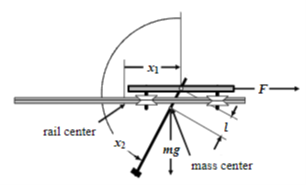
\includegraphics[width=0.55\textwidth]{schemat.png}
    \caption{Schemat układu (źródło: instrukcja dołączona do obiektu)}
    \label{fig:schemat}
\end{figure}

\newpage

\section{Pomiary modelu}

\subsection{Pomiary wahadła}

Przeprowadzono działania mające na celu uzyskanie wartości wagi oraz długości pręta wahadła i obciążnika zamontowanego na jego końcu. Uznano, że druga para wahadła ma takie same wartości parametrów. Odkręcono pręt od wózka, zdjęto obciążk i wykonano pomiary, które wykazały następujące wartości:

\begin{itemize}
    \item długość pręta - 50 cm
    \item długość odważnika - 1.8 cm
    \item odległość od końca pręta do środka ciężkości (wyznaczonego eksperymentalnie) - 33.6 cm
    \item odległość od połowy odważnika do środka ciężkości - 15.5 cm
    \item odległość od punktu obrotu do środka ciężkości - 25 cm
\end{itemize}

Eksperyment, za pomocą którego wyznaczono środek ciężkości polegał na zrównoważeniu poziomo położonego pręta na cienkim obiekcie. Przesuwając pręt w obie strony, udało się uzyskać punkt równowagi, co świadczyło że w tym punkcie znajduje się środek ciężkości pręta.

Za punkt obrotu przyjęty został punkt, w którym było przyłożone mocowanie do wózka. Uznano, że domyślnie wybrany punkt będzie odpowiedni.

Sprawdzanie wszystkich odległości miało zapewnić o poprawności wykonanych pomiarów (co jak można zauważyć zostało spełnione (suma odległości od jednego końca do środa odważnika oraz połowa odważnika jest równa sumarycznej długości pręta)

Wykonano również pomiar masy, wyniki są następujące:
\begin{itemize}
    \item masa pręta - 20 g,
    \item masa obciążnika - 11 g,
    \item masa pręta i obciążnika - 31 g.
\end{itemize}

Tutaj również wykonano sprawdzenie poprawności pomiarów i również dało ono pozytywny wynik.

\subsection{Pomiar siły wytwarzanej przez silnik}\label{subsec:sila_silnik}

W celu wyznaczenia siły wytwarzanej przez silnik, zespół zbadał wartość siły dla zadanych wartości wypełnienia PWM. Przedstawione w tabeli wartości zawierają wypełnienie sygnału PWM, napięcie przyłożone do silnika, siłę z jaką działa silnik na wózek.

\begin{center}
\begin{tabular}{c|c|c}
     Wypełnienie & Napięcie [V] & Siła [F]\\\hline
     0.1 & 2.4 & 1\\\hline
     0.15 & 3.6 & 2.2\\\hline
     0.2 & 4.8 & 3\\\hline
     0.25 & 6 & 3.5\\\hline
     0.3 & 7.2 & 4\\\hline
     0.35 & 8.4 & 4.6\\\hline
     0.4 & 9.6 & 5.3\\\hline
     0.45 & 10.8 & 5.7\\\hline
     0.5 & 12 & 6\\\hline
     0.55 & 12 & 6\\\hline
     0.6 & 12 & 6\\\hline
     0.65 & 12 & 6
\end{tabular}
\end{center}

Można zauważyć w powyższej tabeli pewną nieprawidłowość. Mianowicie dla wypełnienia większego bądź równego 0.5, wartość napięcia ani siły się nie zmienia. Jest to spowodowane ograniczeniem obiektu (zabezpieczeniem), który nie przyjmie większego napięcia niż 12 V, tym samym nie uzyska siły większej niż dla 12 V (tj. 6 N).

\newpage

\section{Wyznaczenie współczynników tarcia}

Podczas laboratorium wykonano eksperymenty pozwalające wyznaczyć zarówno tarcie wiskotyczne (dynamiczne), jak i tarcie statyczne.

\subsection{Eksperyment wahadła}

Dla wahadła wykonano cztery wariacje eksperymentu polegającego na ruchu swobodnym wahadła (\ref{fig:wahadlo45}-\ref{fig:wahadlo180}). Każda z wariacji różniła się zadanym początkowym wyhyleniem. Jednak z racji niskich wartości tarć, zdecydowano się je pominąć, tym samym upraszczając model. Zespół wraz z prowadzącym podjął decyzję, że wpływ tarcia nie będzie znaczący dla systemu sterowania.

\begin{figure}[H]
    \centering
    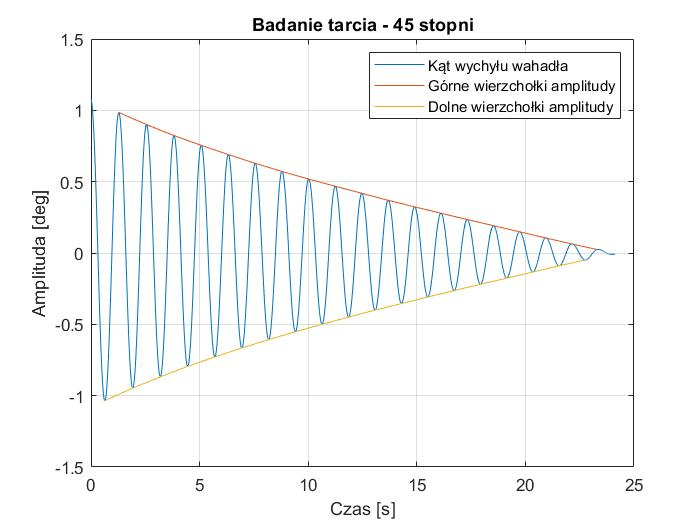
\includegraphics[width=0.95\textwidth]{wahadlo45.jpg}
    \caption{Wykres wychylenia wahadła w czasie dla kąta początkowego - 45°C}
    \label{fig:wahadlo45}
\end{figure}

Obliczony okres drgań wynosi 1.223 s.

\begin{figure}[H]
    \centering
    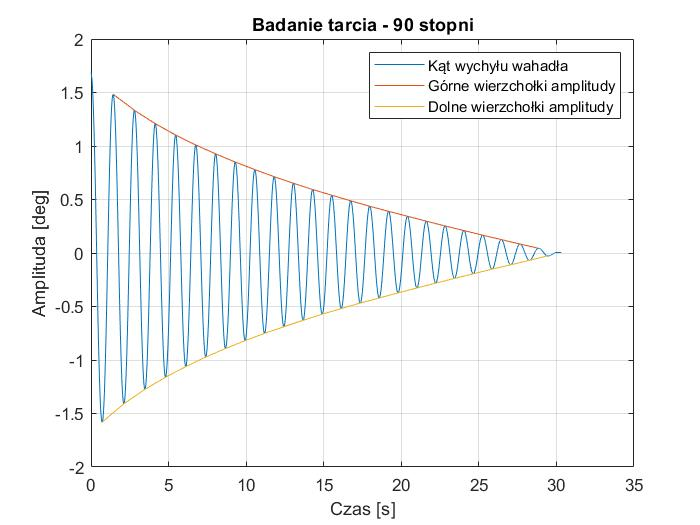
\includegraphics[width=0.95\textwidth]{wahadlo90.jpg}
    \caption{Wykres wychylenia wahadła w czasie dla kąta początkowego - 90°C}
    \label{fig:wahadlo90}
\end{figure}

Obliczony okres drgań wynosi 1.246 s.

\begin{figure}[H]
    \centering
    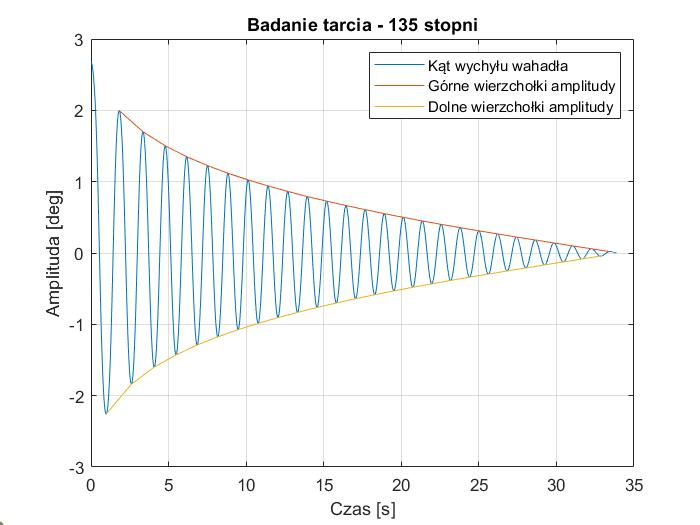
\includegraphics[width=0.95\textwidth]{wahadlo135.jpg}
    \caption{Wykres wychylenia wahadła w czasie dla kąta początkowego - 135°C}
    \label{fig:wahadlo135}
\end{figure}

Obliczony okres drgań wynosi 1.263 s.

\begin{figure}[H]
    \centering
    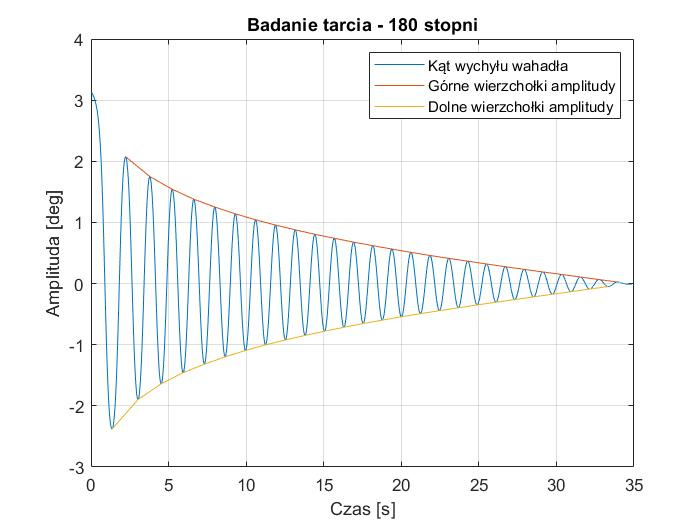
\includegraphics[width=0.95\textwidth]{wahadlo180.jpg}
    \caption{Wykres wychylenia wahadła w czasie dla kąta początkowego - 180°C}
    \label{fig:wahadlo180}
\end{figure}

Obliczony okres drgań wynosi 1.267 s.

Uśredniając uzyskane okresy drgań własnych uzyskano wartość równą 1.25 s.

\subsection{Eksperyment wózka}

Dla wózka przeprowadzono podobny eksperyment (z ruchem swobodnym). Zapisano dane dla współczynników wypełnienia -0.15, 0.15 oraz 0.25, jednak z racji później zauważonych sporych szumów w sygnale prędkości wózka, zdecydowano się wykorzystać wyłącznie pomiary z przyjętego współczynnika 0.25. Przedstawione zostały na rys. \ref{fig:wozek}, \ref{fig:wozek_zoom}.

\begin{figure}[H]
    \centering
    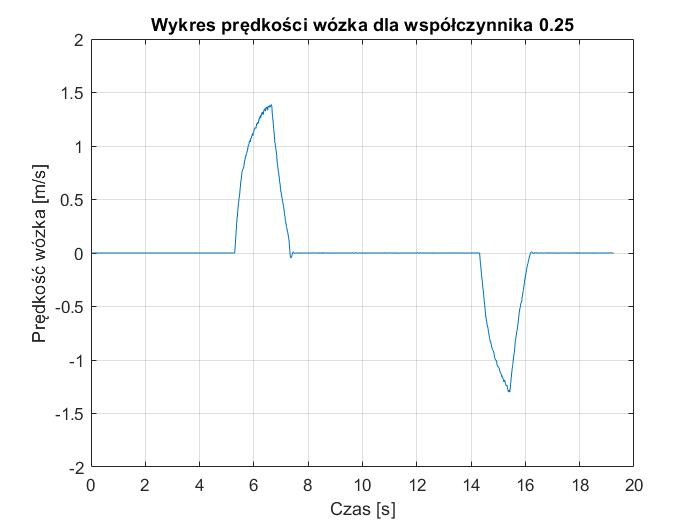
\includegraphics[width=0.95\textwidth]{wozek.jpg}
    \caption{Wykres prędkości wózka dla współczynnika wypełnienia PWM = 0.25}
    \label{fig:wozek}
\end{figure}

By lepiej zobrazować kształt oraz przebieg wykresu, został on przedstawiony w powiększeniu na rys. \ref{fig:wozek_zoom}

\begin{figure}[H]
    \centering
    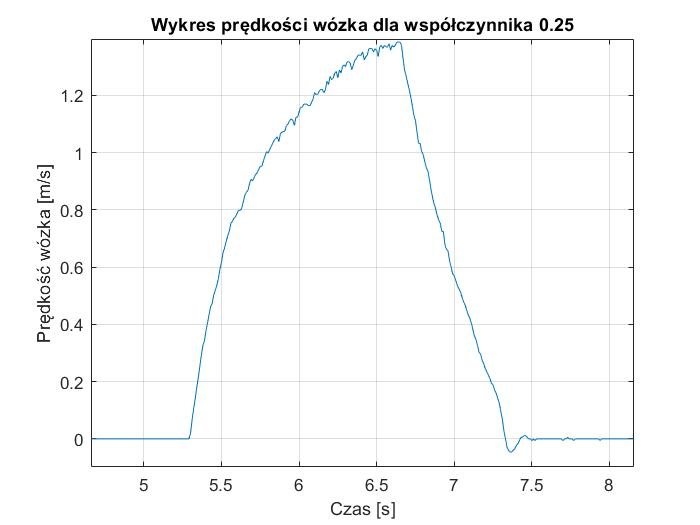
\includegraphics[width=0.95\textwidth]{wozek_zoom.jpg}
    \caption{Wykres prędkości wózka w powiększeniu dla współczynnika wypełnienia PWM = 0.25}
    \label{fig:wozek_zoom}
\end{figure}

Zarówno jak przy współczynnikach tarcia dla wahadła, również tutaj zdecydowano się uznać tarcia za pomijalnie małe.

\subsection{Podsumowanie identyfikacji}

Po przeprowadzeniu identyfikacji parametrów obiektu możliwe było wyznaczenie momentu bezwładności prętów wahadła oraz współczynników tarcia układu - zarówno wózka, jak i wahadła. W podstawowym modelu matematycznym postanowiono nie uwzględniać tarcia - regulator LQR opracowany na podstawie uproszczonego modelu również powinien być w stanie wysterować układ rzeczywisty.

\newpage

\section{Model matematyczny}

Model układu został przedstawiony na rysunku \ref{fig:schemat}. Na tym etapie prac, tarcie wahadła oraz wózka zostało pominięte.

Wartości wykorzystywane w trakcie obliczeń:

\begin{conditions}
    $M$ & masa wózka [kg], \\
    $m$ & masa wahadła [kg], \\
    $L$ & odległość środka masy wahadła od punktu obrotu [m], \\
    $g$ & przyspieszenie grawitacyjne [$\frac{kg*m}{s^{2}}$].
\end{conditions}

\subsection{Dynamika wahadła - uwolnienie od więzów}
W celu wyznaczenia wartości przyspieszeń liniowych i kątowych wahadła, uwolniono od więzów pręt oraz wózek, wskutek czego uzyskano siły reakcji N oraz P. Wynik przedstawiono na rysunkach \ref{fig:wiezy_wozek} i \ref{fig:wiezy_wahadlo}.

\begin{figure}[H]
    \centering
    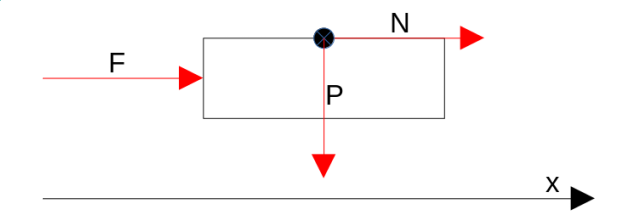
\includegraphics[width=0.6\textwidth]{wiezy_wozek.png}
    \caption{Siły działające na wózek po uwolnieniu od więzów}
    \label{fig:wiezy_wozek}
\end{figure}

Siły P i N działają odpowiednio wzdłuż osi OY i OX, są one reakcjami, opisanymi na początku tego podrozdziału.

\begin{figure}[H]
    \centering
    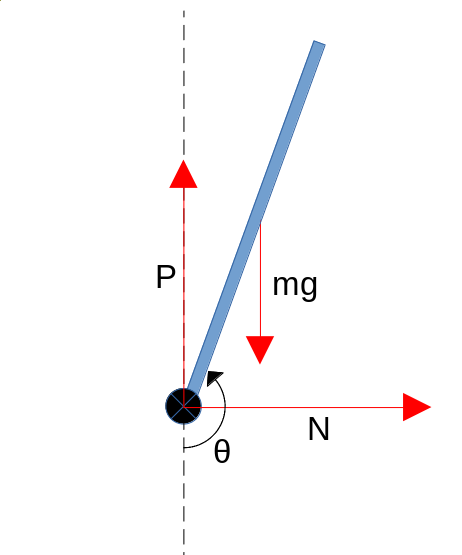
\includegraphics[width=0.6\textwidth]{wiezy_wahadlo.png}
    \caption{Siły działające na wahadło po uwolnieniu od więzów}
    \label{fig:wiezy_wahadlo}
\end{figure}

Po uwolnieniu od więzów przystąpiono do wyznaczenia równań dynamiki dla wózka (\ref{eq:dynamika_wozka_x}) oraz wahadła (\ref{eq:dynamika_wahadla_moment}):

\begin{align}
    M\Ddot{x} &= \sum{F_{ix}} = F - N \label{eq:dynamika_wozka_x}\\
    J\Ddot{\theta} &= \sum{M_{s}} = -PL\sin{\theta} - NL\cos{\theta} \label{eq:dynamika_wahadla_moment}
\end{align}

W przypadku wózka wyliczane jest tylko przyspieszenie wzdłuż osi OX, zaś w przypadku wahadła - przyspieszenie kątowe, gdyż cały układ ma 2 stopnie swobody - właśnie położenie $x$ i położenie kątowe $\theta$.

\subsection{Analiza sił reakcji}

Aby dokładnie określić ruch wahadła, należy rozważyć układ sił działających na wahadło (\ref{eq:dynamika_wahadla_x}, \ref{eq:dynamika_wahadla_y}):

\begin{align}
    m\Ddot{x_{p}} &= N \label{eq:dynamika_wahadla_x}\\
    m\Ddot{y_{p}} &= P - mg \label{eq:dynamika_wahadla_y}
\end{align}

Przyspieszenia liniowe wahadła $\Ddot{x_{p}}$ i $\Ddot{y_{p}}$ wyznaczono na podstawie kinematyki układu (\ref{eq:kinematyka_start} - \ref{eq:kinematyka_stop}):

\begin{align}
    x_{p} &= x + L\sin{\theta} \label{eq:kinematyka_start}\\
    \dot{x_{p}} &= \dot{x} + L\dot{\theta}\cos{\theta} \\
    \Ddot{x_{p}} &= \Ddot{x} - L\dot{\theta}^{2}\sin{\theta} + L\Ddot{\theta}\cos{\theta}\label{eq:x_wah_przyspieszenie} \\
    y_{p} &= -L\cos{\theta} \\
    \dot{y_{p}} &= L\dot{\theta}\sin{\theta} \\
    \Ddot{y_{p}} &= L\dot{\theta}^{2}\cos{\theta} + L\Ddot{\theta}\sin{\theta}\label{eq:kinematyka_stop}
\end{align}

Wykorzystując wyliczone wyżej przyspieszenia (\ref{eq:x_wah_przyspieszenie}) i (\ref{eq:kinematyka_stop}), wyznaczono wzory na wartość sił P i N (\ref{eq:p_wzor}, \ref{eq:n_wzor}):

\begin{align}
    N &= m(\Ddot{x} - L\dot{\theta}^{2}\sin{\theta} + L\Ddot{\theta}\cos{\theta}) \label{eq:n_wzor} \\
    P &= m(L\dot{\theta}^{2}\cos{\theta} + L\Ddot{\theta}\sin{\theta} + g) \label{eq:p_wzor}
\end{align}

Równania sił (\ref{eq:n_wzor}) i (\ref{eq:p_wzor}) wstawiono do równań (\ref{eq:dynamika_wozka_x}) oraz (\ref{eq:dynamika_wahadla_moment}), uzyskując ostateczne równania dynamiki układu (\ref{eq:dynamika_ost_x}) i (\ref{eq:dynamika_ost_theta}):

\begin{align}
    &(M+M)\Ddot{x} + mL\Ddot{\theta}\cos{\theta} - mL\dot{\theta}^{2}\sin{\theta} = F \label{eq:dynamika_ost_x}\\
    &(J+mL^{2})\Ddot{\theta} + mgL\sin{\theta} = -mL\Ddot{x}\cos{\theta} \label{eq:dynamika_ost_theta}
\end{align}

Równania (\ref{eq:dynamika_ost_x}) i (\ref{eq:dynamika_ost_theta}) przekształcono następnie tak, aby uzyskać wzory na przyspieszenia liniowe i kątowe (\ref{eq:przyspieszenie_x}), (\ref{eq:przyspieszenie_theta}):

\begin{align}
\Ddot{x} &= \frac{m^{2}gL^{2}\sin{\theta}\cos{\theta} + mL(J + mL^{2})\dot{\theta}^{2}\sin{\theta} + (J+ mL^{2}) * F}{J(M + m) + mML^{2} + m^{2}L^{2}\sin^{2}{\theta}} \label{eq:przyspieszenie_x} \\
    \Ddot{\theta} &= \frac{-(M + m)mgL\sin{\theta} - mL\cos{\theta}*F - m^{2}L^{2}\dot{\theta}^{2}\sin{\theta}\cos{\theta}}{J(M + m) + mML^{2} + m^{2}L^{2}\sin^{2}{\theta}} \label{eq:przyspieszenie_theta}
\end{align}

\subsection{Nieliniowe równania stanu}

Wzory przyspieszeń służą do wyprowadzenia nieliniowych równań stanu. Przyjęto następujący wektor stanu (\ref{eq:wektor_stanu}):

\begin{equation}
    \textbf{x} = \left[x_{1} \hspace{5px} x_{2} \hspace{5px} x_{3} \hspace{5px} x_{4}\right]^T = \left[x \hspace{5px} \dot{x} \hspace{5px} \theta \hspace{5px} \dot{\theta}\right]^T \label{eq:wektor_stanu}
\end{equation}

Z wykorzystaniem równań (\ref{eq:przyspieszenie_x}), (\ref{eq:przyspieszenie_theta}) i (\ref{eq:wektor_stanu}) wyprowadzono nieliniowe równania stanu, opisujące zależności pomiędzy wahadłem a wózkiem.

\begin{align}
    \dot{x_{1}} &= x_{2} \\
    \dot{x_{2}} &= \frac{m^{2}gL^{2}\sin{x_{3}}\cos{x_{3}} + mL(J + mL^{2})\dot{x_{3}}^{2}\sin{x_{3}} + (J+ mL^{2}) * F}{J(M + m) + mML^{2} + m^{2}L^{2}\sin^{2}{x_{3}}} \\
    \dot{x_{3}} &= x_{4} \\
    \dot{x_{4}} & = \frac{-(M + m)mgL\sin{x_{3}} - mL\cos{x_{3}}*F - m^{2}L^{2}\dot{x_{3}}^{2}\sin{x_{3}}\cos{x_{3}}}{J(M + m) + mML^{2} + m^{2}L^{2}\sin^{2}{x_{3}}}
\end{align}

Na podstawie doświadczeń z podrozdziału \ref{subsec:sila_silnik}, siła F wyrażona jest następującym wzorem: 

\begin{equation}
    F = 0.5*u + 0.3 \label{eq:wzor_sila_sterowanie}
\end{equation}

Gdzie $u$ to napięcie sterujące z zakresu $\pm 12V$.

Po podstawieniu (\ref{eq:wzor_sila_sterowanie}) do równań stanu, uzyskano następujące równania:

\begin{align}
    \dot{x_{1}} &= x_{2} \\
    \dot{x_{2}} &= \frac{m^{2}gL^{2}\sin{x_{3}}\cos{x_{3}} + mL(J + mL^{2})x_{4}^{2}\sin{x_{3}} + (J+ mL^{2}) * (0.5*u + 0.3)}{J(M + m) + mML^{2} + m^{2}L^{2}\sin^{2}{x_{3}}} \\
    \dot{x_{3}} &= x_{4} \\
    \dot{x_{4}} & = \frac{-(M + m)mgL\sin{x_{3}} - mL\cos{x_{3}}*(0.5*u + 0.3) - m^{2}L^{2}x_{4}^{2}\sin{x_{3}}\cos{x_{3}}}{J(M + m) + mML^{2} + m^{2}L^{2}\sin^{2}{x_{3}}}
\end{align}

\subsection{Linearyzacja równań stanu}

Linearyzację układu przeprowadzono wokół punktu równowagi $\theta = \pi$. Wskutek tego założenia, możliwe jest przybliżenie wartości funkcji trygonometrycznych:

\begin{align*}
    \sin{\theta} &\approx -\theta \\
    \cos{\theta} &\approx -1 \\
    \sin{2\theta} &\approx 2\theta
\end{align*}

Po linearyzacji, uzyskano następujące równania stanu:

\begin{align}
    \dot{x_{1}} &= x_{2} \\
    \dot{x_{2}} &= \frac{m^{2}gL^{2}x_{3} + (J+ mL^{2}) * (0.5*u + 0.3)}{J(M + m) + mML^{2}} \\
    \dot{x_{3}} &= x_{4} \\
    \dot{x_{4}} & = \frac{(M + m)mgLx_{3} + mL*(0.5*u + 0.3)}{J(M + m) + mML^{2}}
\end{align}

Zlinearyzowane równania stanu zostały wykorzystanie do utworzenia modelu symulacyjnego wahadła odwróconego.

\section{Model symulacyjny}

Na podstawie modelu matematycznego został utworzony model symulacyjny w Simulinku (\ref{fig:model_symulacyjny}).

\begin{figure}[H]
    \centering
    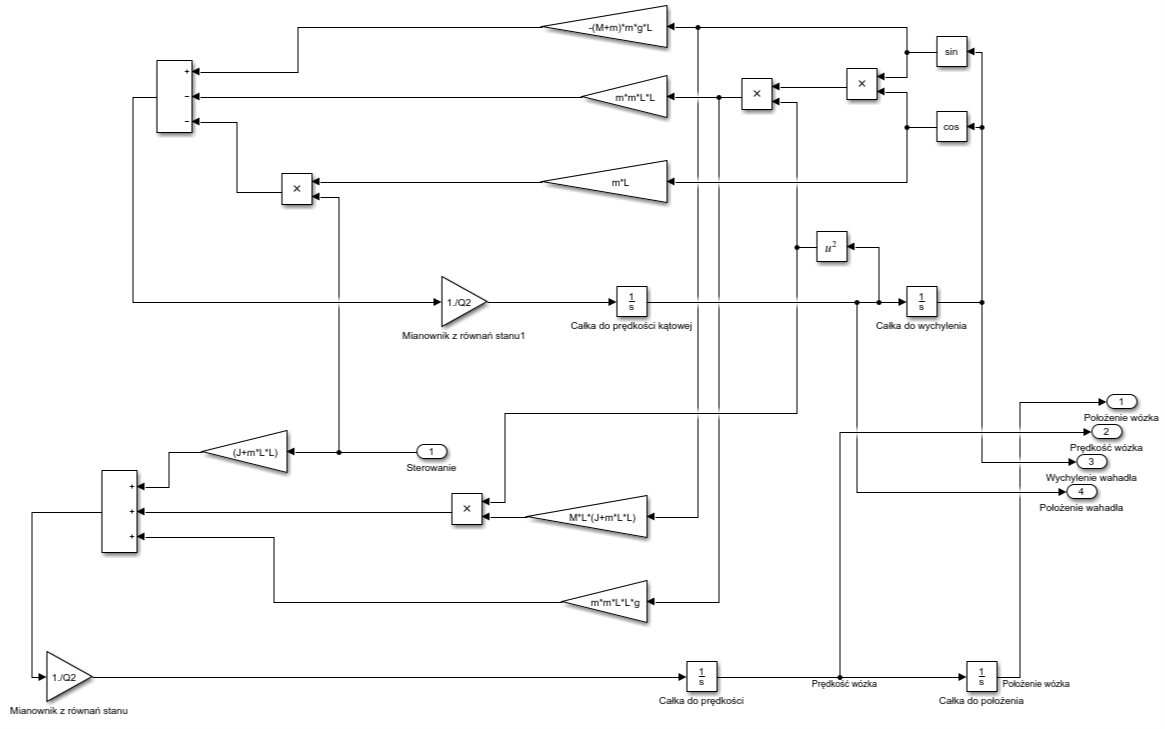
\includegraphics[width=0.6\textwidth]{model_sym.png}
    \caption{Model symulacyjny wahadła odwróconego}
    \label{fig:model_symulacyjny}
\end{figure}

Został on dołączony do istniejącej aplikacji sterującej wózkiem. Dodatkowo została dodana histereza w zależności od położenia wózka. Rozwiązanie to pozwoli uniknąć sytuacji, w której wózek uderza w krawędź szyny. Na podstawie sygnału położenia wózka (rys. \ref{fig:histereza}) sprawdzane są warunki ze stałymi wartościami granicznymi, po przekroczeniu których wózek przez chwilę porusza się z maksymalną prędkością w przeciwnym kierunku, żeby zapobiec zderzeniu wózka z krawędzią szyny.

\begin{figure}[H]
    \centering
    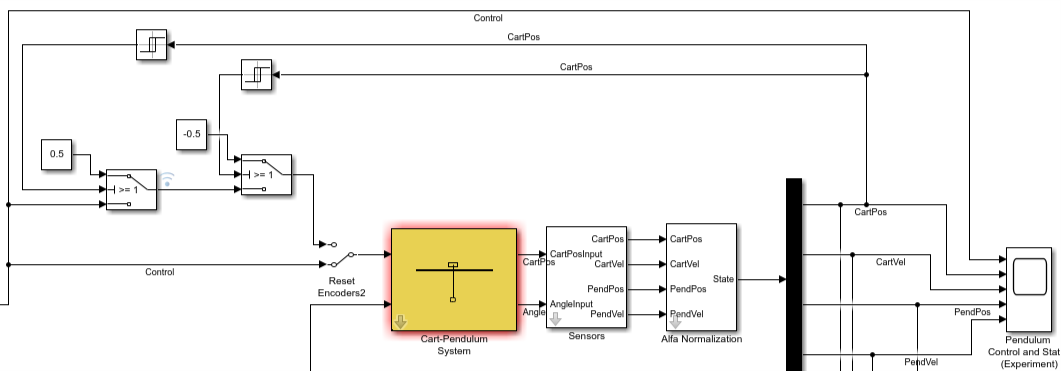
\includegraphics[width=0.6\textwidth]{histereza.png}
    \caption{Fragment schematu symulacji z wyszczególnionym modułem histerezy}
    \label{fig:histereza}
\end{figure}

\section{Regulator LQR}

Równanie regulatora (\ref{eq:wzor_LQR}) będzie wykorzystane jako sterowanie w układzie.

\begin{equation}
    u(t) = -Kx(t)
    \label{eq:wzor_LQR}
\end{equation}

Równaniem decydującym o wartościach macierzy K było równanie \ref{eq:wzor_matrix1}, z którego otrzymano zależność \ref{eq:wzor_LQR_x_prim}

\begin{align}
    \dot{x} &= Ax(t) + Bu(t) \label{eq:wzor_matrix1}\\
    y &= Cx(t) + Du(t) \label{eq:wzor_matrix2}
\end{align}

\begin{align}
\label{eq:wzor_LQR_x_prim}
    \dot{x} &= Ax(t) + BKx(t)\\
    \dot{x} &= (A + BK) x(t)
\end{align}

Na podstawie zadanych wartości uchybu oraz wartości sterowania uzyskano macierze obserwatora (\ref{mat:Q}) i regulatora (\ref{mat:R}). Wykorzystując macierze A, B, Q i R obliczono macierz wzmocnień K (\ref{mat:K}).

\begin{align}
    Q &= \begin{bmatrix} 
    100 & 0 & 0 & 0\\
    0 & 100 & 0 & 0\\
    0 & 0 & 3600 & 0\\
    0 & 0 & 0 & 100\end{bmatrix} \label{mat:Q}\\
    R &= 0.5 \label{mat:R} \\
    K &= \begin{bmatrix}
    -10.00 & -19.92 & 161.95 & 49.60\end{bmatrix} \label{mat:K} \\
\end{align}

Zaimplementowany regulator został dodany do modelu symulacyjnego oraz przedstawiony na rys. \ref{fig:lqr}

\begin{figure}[H]
    \centering
    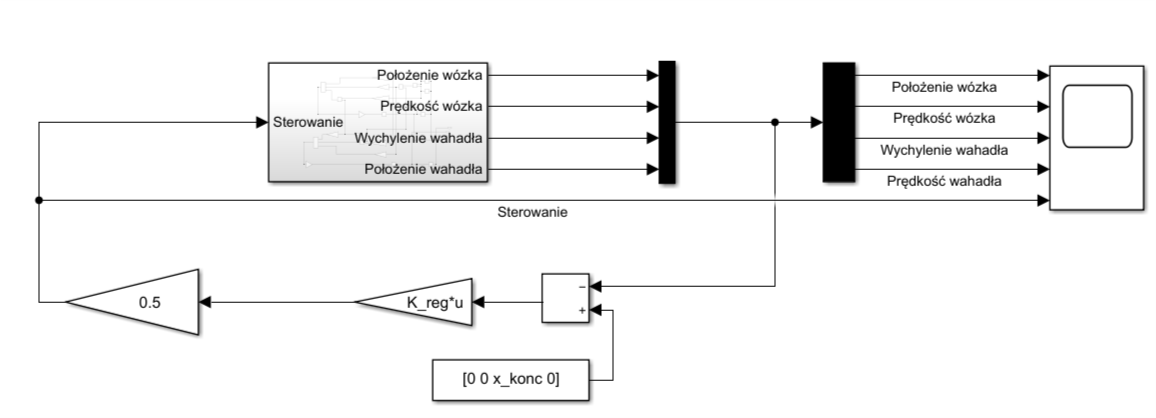
\includegraphics[width=0.6\textwidth]{lqr.png}
    \caption{Model symulacyjny wahadła odwróconego z regulatorem LQR}
    \label{fig:lqr}
\end{figure}

\section{Testowanie na obiekcie rzeczywistym}

W trakcie testowania obliczonego regulatora na obiekcie rzeczywistym, ujawnione zostały problemy związane z błędnym przyjęciem zwrotu kąta $\theta$ - w obiekcie rzeczywistym $\theta$ ma zwrot zgodnie z ruchem wskazówek zegara, w obiekcie modelowanym - przeciwnie do wskazówek zegara. W celu poprawy implementacji, wymagana jest korekcja znaku kąta - jest to realizowalne na jeden z dwóch sposobów:

\begin{itemize}
    \item odwrócenie znaku wyjściowej wartości kąta z obiektu,
    \item zmiana kierunku kąta $\theta$ w modelu matematycznym.
\end{itemize}

Sposób rozwiązania napotkanego problemu zostanie dobrany w ciągu najbliższych zajęć. Ponadto, wymagane jest opracowanie mechanizmu swing-up, w celu doprowadzenia wahadła do punktu zbliżonego do punktu równowagi, gdyż tylko w jego otoczeniu realizowana jest regulacja.

% \section{Moduł Swing-Up}

% \section{Weryfikacja}

\end{document}
